\documentclass[twoside]{book}

% Packages required by doxygen
\usepackage{fixltx2e}
\usepackage{calc}
\usepackage{doxygen}
\usepackage[export]{adjustbox} % also loads graphicx
\usepackage{graphicx}
\usepackage[utf8]{inputenc}
\usepackage{makeidx}
\usepackage{multicol}
\usepackage{multirow}
\PassOptionsToPackage{warn}{textcomp}
\usepackage{textcomp}
\usepackage[nointegrals]{wasysym}
\usepackage[table]{xcolor}

% Font selection
\usepackage[T1]{fontenc}
\usepackage[scaled=.90]{helvet}
\usepackage{courier}
\usepackage{amssymb}
\usepackage{sectsty}
\renewcommand{\familydefault}{\sfdefault}
\allsectionsfont{%
  \fontseries{bc}\selectfont%
  \color{darkgray}%
}
\renewcommand{\DoxyLabelFont}{%
  \fontseries{bc}\selectfont%
  \color{darkgray}%
}
\newcommand{\+}{\discretionary{\mbox{\scriptsize$\hookleftarrow$}}{}{}}

% Page & text layout
\usepackage{geometry}
\geometry{%
  letterpaper,%
  top=2.5cm,%
  bottom=2.5cm,%
  left=2.5cm,%
  right=2.5cm%
}
\tolerance=750
\hfuzz=15pt
\hbadness=750
\setlength{\emergencystretch}{15pt}
\setlength{\parindent}{0cm}
\setlength{\parskip}{3ex plus 2ex minus 2ex}
\makeatletter
\renewcommand{\paragraph}{%
  \@startsection{paragraph}{4}{0ex}{-1.0ex}{1.0ex}{%
    \normalfont\normalsize\bfseries\SS@parafont%
  }%
}
\renewcommand{\subparagraph}{%
  \@startsection{subparagraph}{5}{0ex}{-1.0ex}{1.0ex}{%
    \normalfont\normalsize\bfseries\SS@subparafont%
  }%
}
\makeatother

% Headers & footers
\usepackage{fancyhdr}
\pagestyle{fancyplain}
\fancyhead[LE]{\fancyplain{}{\bfseries\thepage}}
\fancyhead[CE]{\fancyplain{}{}}
\fancyhead[RE]{\fancyplain{}{\bfseries\leftmark}}
\fancyhead[LO]{\fancyplain{}{\bfseries\rightmark}}
\fancyhead[CO]{\fancyplain{}{}}
\fancyhead[RO]{\fancyplain{}{\bfseries\thepage}}
\fancyfoot[LE]{\fancyplain{}{}}
\fancyfoot[CE]{\fancyplain{}{}}
\fancyfoot[RE]{\fancyplain{}{\bfseries\scriptsize Generated by Doxygen }}
\fancyfoot[LO]{\fancyplain{}{\bfseries\scriptsize Generated by Doxygen }}
\fancyfoot[CO]{\fancyplain{}{}}
\fancyfoot[RO]{\fancyplain{}{}}
\renewcommand{\footrulewidth}{0.4pt}
\renewcommand{\chaptermark}[1]{%
  \markboth{#1}{}%
}
\renewcommand{\sectionmark}[1]{%
  \markright{\thesection\ #1}%
}

% Indices & bibliography
\usepackage{natbib}
\usepackage[titles]{tocloft}
\setcounter{tocdepth}{3}
\setcounter{secnumdepth}{5}
\makeindex

% Hyperlinks (required, but should be loaded last)
\usepackage{ifpdf}
\ifpdf
  \usepackage[pdftex,pagebackref=true]{hyperref}
\else
  \usepackage[ps2pdf,pagebackref=true]{hyperref}
\fi
\hypersetup{%
  colorlinks=true,%
  linkcolor=blue,%
  citecolor=blue,%
  unicode%
}

% Custom commands
\newcommand{\clearemptydoublepage}{%
  \newpage{\pagestyle{empty}\cleardoublepage}%
}

\usepackage{caption}
\captionsetup{labelsep=space,justification=centering,font={bf},singlelinecheck=off,skip=4pt,position=top}

%===== C O N T E N T S =====

\begin{document}

% Titlepage & ToC
\hypersetup{pageanchor=false,
             bookmarksnumbered=true,
             pdfencoding=unicode
            }
\pagenumbering{roman}
\begin{titlepage}
\vspace*{7cm}
\begin{center}%
{\Large R\+LG 327 File Parser \\[1ex]\large 0.\+0.\+1 }\\
\vspace*{1cm}
{\large Generated by Doxygen 1.8.11}\\
\end{center}
\end{titlepage}
\clearemptydoublepage
\tableofcontents
\clearemptydoublepage
\pagenumbering{arabic}
\hypersetup{pageanchor=true}

%--- Begin generated contents ---
\chapter{Module Index}
\section{Modules}
Here is a list of all modules\+:\begin{DoxyCompactList}
\item \contentsline{section}{Vespertiine}{\pageref{group__vespertiine}}{}
\end{DoxyCompactList}

\chapter{Namespace Index}
\section{Namespace List}
Here is a list of all namespaces with brief descriptions\+:\begin{DoxyCompactList}
\item\contentsline{section}{\hyperlink{namespacevespertiine}{vespertiine} }{\pageref{namespacevespertiine}}{}
\end{DoxyCompactList}

\chapter{Class Index}
\section{Class List}
Here are the classes, structs, unions and interfaces with brief descriptions\+:\begin{DoxyCompactList}
\item\contentsline{section}{\hyperlink{classvespertiine_1_1FileParser}{vespertiine\+::\+File\+Parser} \\*Parses C\+OM S 327 D\+IF files to a vector of maps of string pairs }{\pageref{classvespertiine_1_1FileParser}}{}
\end{DoxyCompactList}

\chapter{File Index}
\section{File List}
Here is a list of all files with brief descriptions\+:\begin{DoxyCompactList}
\item\contentsline{section}{src/\hyperlink{FileParser_8cpp}{File\+Parser.\+cpp} }{\pageref{FileParser_8cpp}}{}
\item\contentsline{section}{src/\hyperlink{runner_8cpp}{runner.\+cpp} }{\pageref{runner_8cpp}}{}
\item\contentsline{section}{src/include/\hyperlink{FileParser_8hpp}{File\+Parser.\+hpp} }{\pageref{FileParser_8hpp}}{}
\end{DoxyCompactList}

\chapter{Module Documentation}
\hypertarget{group__vespertiine}{}\section{Vespertiine}
\label{group__vespertiine}\index{Vespertiine@{Vespertiine}}
\subsection*{Namespaces}
\begin{DoxyCompactItemize}
\item 
 \hyperlink{namespacevespertiine}{vespertiine}
\end{DoxyCompactItemize}
\subsection*{Classes}
\begin{DoxyCompactItemize}
\item 
class \hyperlink{classvespertiine_1_1FileParser}{vespertiine\+::\+File\+Parser}
\begin{DoxyCompactList}\small\item\em Parses C\+OM S 327 D\+IF files to a vector of maps of string pairs. \end{DoxyCompactList}\end{DoxyCompactItemize}
\subsection*{Typedefs}
\begin{DoxyCompactItemize}
\item 
using \hyperlink{group__vespertiine_ga7e5191e67b3b71f8044b653a3f9b2065}{vespertiine\+::string} = std\+::string
\item 
using \hyperlink{group__vespertiine_ga338498d8eeb1f5a3da1f237df24c4250}{vespertiine\+::istream} = std\+::istream
\item 
using \hyperlink{group__vespertiine_ga01f4e06d9363d6dc31a69d8a0553b93d}{vespertiine\+::entity\+\_\+vector} = std\+::vector$<$ entity $>$
\item 
using \hyperlink{group__vespertiine_ga39a811996b190f9e1ffa0663d4f5744a}{vespertiine\+::file\+\_\+key} = std\+::string
\item 
using \hyperlink{group__vespertiine_ga546be9d1b39ff78c5bf63e598bc51a0a}{vespertiine\+::file\+\_\+value} = std\+::string
\item 
using \hyperlink{group__vespertiine_gaf9205d715bdeade18d7039864ef59b44}{vespertiine\+::entity} = std\+::map$<$ file\+\_\+key, file\+\_\+value $>$
\item 
using \hyperlink{group__vespertiine_ga1294ff353dd9ea9b26cf4a1573db109e}{vespertiine\+::file\+\_\+header} = std\+::pair$<$ std\+::string, unsigned int $>$
\end{DoxyCompactItemize}
\subsection*{Functions}
\begin{DoxyCompactItemize}
\item 
std\+::ostream \& \hyperlink{group__vespertiine_ga1ca507e4b8f52201ba9cccaaf496e9be}{vespertiine\+::operator$<$$<$} (std\+::ostream \&output, const \hyperlink{classvespertiine_1_1FileParser}{vespertiine\+::\+File\+Parser} \&F)
\item 
\hyperlink{group__vespertiine_ga01e372573c11d4c2848419c8842d583e}{vespertiine\+::\+File\+Parser\+::\+File\+Parser} (std\+::string file\+\_\+path)
\begin{DoxyCompactList}\small\item\em Construct and populate the \hyperlink{classvespertiine_1_1FileParser}{File\+Parser}. \end{DoxyCompactList}\item 
\hyperlink{group__vespertiine_gad562ef6be958292fbc74803d47b0eda3}{vespertiine\+::\+File\+Parser\+::\+File\+Parser} (std\+::vector$<$ entity $>$ entities, std\+::string entity\+\_\+type, std\+::string file\+\_\+type, unsigned int version\+\_\+number)
\begin{DoxyCompactList}\small\item\em Construct a \hyperlink{classvespertiine_1_1FileParser}{File\+Parser} based on an existing entity. \end{DoxyCompactList}\item 
const std\+::vector$<$ entity $>$ \hyperlink{group__vespertiine_gac2360eb7febe37b75f13dc697a3d37ed}{vespertiine\+::\+File\+Parser\+::get\+Entities} () const 
\begin{DoxyCompactList}\small\item\em Return the contents of the file. \end{DoxyCompactList}\item 
const unsigned int \hyperlink{group__vespertiine_ga69070e93ff23a24380d0bad1c096205a}{vespertiine\+::\+File\+Parser\+::get\+File\+Version} () const 
\begin{DoxyCompactList}\small\item\em Return the version of the file as a single unsigned integer. \end{DoxyCompactList}\item 
const std\+::string \hyperlink{group__vespertiine_ga950b19f6ead99d8297e37eaeeed2fd3f}{vespertiine\+::\+File\+Parser\+::get\+File\+Type} () const 
\begin{DoxyCompactList}\small\item\em Return the type of the file as a string. \end{DoxyCompactList}\end{DoxyCompactItemize}
\subsection*{Friends}
\begin{DoxyCompactItemize}
\item 
std\+::ostream \& \hyperlink{group__vespertiine_ga6d174b85be314a05d54a9d63a7f1fbbb}{vespertiine\+::\+File\+Parser\+::operator$<$$<$} (std\+::ostream \&output, const File\+Parser \&F)
\begin{DoxyCompactList}\small\item\em Overload the output operator to match the style of the D\+IF type. \end{DoxyCompactList}\end{DoxyCompactItemize}


\subsection{Detailed Description}


\subsection{Typedef Documentation}
\index{Vespertiine@{Vespertiine}!entity@{entity}}
\index{entity@{entity}!Vespertiine@{Vespertiine}}
\subsubsection[{\texorpdfstring{entity}{entity}}]{\setlength{\rightskip}{0pt plus 5cm}using {\bf vespertiine\+::entity} = typedef std\+::map$<$file\+\_\+key,file\+\_\+value$>$}\hypertarget{group__vespertiine_gaf9205d715bdeade18d7039864ef59b44}{}\label{group__vespertiine_gaf9205d715bdeade18d7039864ef59b44}


Definition at line 14 of file File\+Parser.\+hpp.

\index{Vespertiine@{Vespertiine}!entity\+\_\+vector@{entity\+\_\+vector}}
\index{entity\+\_\+vector@{entity\+\_\+vector}!Vespertiine@{Vespertiine}}
\subsubsection[{\texorpdfstring{entity\+\_\+vector}{entity_vector}}]{\setlength{\rightskip}{0pt plus 5cm}using {\bf vespertiine\+::entity\+\_\+vector} = typedef std\+::vector$<$entity$>$}\hypertarget{group__vespertiine_ga01f4e06d9363d6dc31a69d8a0553b93d}{}\label{group__vespertiine_ga01f4e06d9363d6dc31a69d8a0553b93d}


Definition at line 21 of file File\+Parser.\+cpp.

\index{Vespertiine@{Vespertiine}!file\+\_\+header@{file\+\_\+header}}
\index{file\+\_\+header@{file\+\_\+header}!Vespertiine@{Vespertiine}}
\subsubsection[{\texorpdfstring{file\+\_\+header}{file_header}}]{\setlength{\rightskip}{0pt plus 5cm}using {\bf vespertiine\+::file\+\_\+header} = typedef std\+::pair$<$std\+::string, unsigned int$>$}\hypertarget{group__vespertiine_ga1294ff353dd9ea9b26cf4a1573db109e}{}\label{group__vespertiine_ga1294ff353dd9ea9b26cf4a1573db109e}


Definition at line 15 of file File\+Parser.\+hpp.

\index{Vespertiine@{Vespertiine}!file\+\_\+key@{file\+\_\+key}}
\index{file\+\_\+key@{file\+\_\+key}!Vespertiine@{Vespertiine}}
\subsubsection[{\texorpdfstring{file\+\_\+key}{file_key}}]{\setlength{\rightskip}{0pt plus 5cm}using {\bf vespertiine\+::file\+\_\+key} = typedef std\+::string}\hypertarget{group__vespertiine_ga39a811996b190f9e1ffa0663d4f5744a}{}\label{group__vespertiine_ga39a811996b190f9e1ffa0663d4f5744a}


Definition at line 12 of file File\+Parser.\+hpp.

\index{Vespertiine@{Vespertiine}!file\+\_\+value@{file\+\_\+value}}
\index{file\+\_\+value@{file\+\_\+value}!Vespertiine@{Vespertiine}}
\subsubsection[{\texorpdfstring{file\+\_\+value}{file_value}}]{\setlength{\rightskip}{0pt plus 5cm}using {\bf vespertiine\+::file\+\_\+value} = typedef std\+::string}\hypertarget{group__vespertiine_ga546be9d1b39ff78c5bf63e598bc51a0a}{}\label{group__vespertiine_ga546be9d1b39ff78c5bf63e598bc51a0a}


Definition at line 13 of file File\+Parser.\+hpp.

\index{Vespertiine@{Vespertiine}!istream@{istream}}
\index{istream@{istream}!Vespertiine@{Vespertiine}}
\subsubsection[{\texorpdfstring{istream}{istream}}]{\setlength{\rightskip}{0pt plus 5cm}using {\bf vespertiine\+::istream} = typedef std\+::istream}\hypertarget{group__vespertiine_ga338498d8eeb1f5a3da1f237df24c4250}{}\label{group__vespertiine_ga338498d8eeb1f5a3da1f237df24c4250}


Definition at line 20 of file File\+Parser.\+cpp.

\index{Vespertiine@{Vespertiine}!string@{string}}
\index{string@{string}!Vespertiine@{Vespertiine}}
\subsubsection[{\texorpdfstring{string}{string}}]{\setlength{\rightskip}{0pt plus 5cm}using {\bf vespertiine\+::string} = typedef std\+::string}\hypertarget{group__vespertiine_ga7e5191e67b3b71f8044b653a3f9b2065}{}\label{group__vespertiine_ga7e5191e67b3b71f8044b653a3f9b2065}


Definition at line 19 of file File\+Parser.\+cpp.



\subsection{Function Documentation}
\index{Vespertiine@{Vespertiine}!File\+Parser@{File\+Parser}}
\index{File\+Parser@{File\+Parser}!Vespertiine@{Vespertiine}}
\subsubsection[{\texorpdfstring{File\+Parser(std\+::string file\+\_\+path)}{FileParser(std::string file_path)}}]{\setlength{\rightskip}{0pt plus 5cm}vespertiine\+::\+File\+Parser\+::\+File\+Parser (
\begin{DoxyParamCaption}
\item[{std\+::string}]{file\+\_\+path}
\end{DoxyParamCaption}
)}\hypertarget{group__vespertiine_ga01e372573c11d4c2848419c8842d583e}{}\label{group__vespertiine_ga01e372573c11d4c2848419c8842d583e}


Construct and populate the \hyperlink{classvespertiine_1_1FileParser}{File\+Parser}. 

The constructor runs the entire program using a private runner() function. It will populate the private entity vector which can then be accessed using \hyperlink{group__vespertiine_gac2360eb7febe37b75f13dc697a3d37ed}{get\+Entities()}.


\begin{DoxyParams}[1]{Parameters}
\mbox{\tt in}  & {\em file\+\_\+path} & A file path string. \\
\hline
\end{DoxyParams}
\begin{DoxyWarning}{Warning}
Will throw std\+::invalid\+\_\+argument exception if any of the filetype assumptions are violated. 
\end{DoxyWarning}


Definition at line 23 of file File\+Parser.\+cpp.

\index{Vespertiine@{Vespertiine}!File\+Parser@{File\+Parser}}
\index{File\+Parser@{File\+Parser}!Vespertiine@{Vespertiine}}
\subsubsection[{\texorpdfstring{File\+Parser(std\+::vector$<$ entity $>$ entities, std\+::string entity\+\_\+type, std\+::string file\+\_\+type, unsigned int version\+\_\+number)}{FileParser(std::vector< entity > entities, std::string entity_type, std::string file_type, unsigned int version_number)}}]{\setlength{\rightskip}{0pt plus 5cm}vespertiine\+::\+File\+Parser\+::\+File\+Parser (
\begin{DoxyParamCaption}
\item[{std\+::vector$<$ {\bf entity} $>$}]{entities, }
\item[{std\+::string}]{entity\+\_\+type, }
\item[{std\+::string}]{file\+\_\+type, }
\item[{unsigned int}]{version\+\_\+number}
\end{DoxyParamCaption}
)}\hypertarget{group__vespertiine_gad562ef6be958292fbc74803d47b0eda3}{}\label{group__vespertiine_gad562ef6be958292fbc74803d47b0eda3}


Construct a \hyperlink{classvespertiine_1_1FileParser}{File\+Parser} based on an existing entity. 

This will convert all of the keys in the entities vector, the entity type, and the file type to uppercase and bind it to a \hyperlink{classvespertiine_1_1FileParser}{File\+Parser}. As such, you can echo back out to file.


\begin{DoxyParams}[1]{Parameters}
\mbox{\tt in}  & {\em entities} & A vector of type entity, which should be a map of string pairs. \\
\hline
\mbox{\tt in}  & {\em entity\+\_\+type} & The type of the entities in the vector, e.\+g. M\+O\+N\+S\+T\+ER, which will be trimmed to one word and capitalized. \\
\hline
\mbox{\tt in}  & {\em file\+\_\+type} & The type of the file, e.\+g. D\+E\+S\+C\+R\+I\+P\+T\+I\+ON, which will be trimmed to one word and capitalized. \\
\hline
\mbox{\tt in}  & {\em version\+\_\+number} & The version, e.\+g. 1. \\
\hline
\end{DoxyParams}


Definition at line 30 of file File\+Parser.\+cpp.

\index{Vespertiine@{Vespertiine}!get\+Entities@{get\+Entities}}
\index{get\+Entities@{get\+Entities}!Vespertiine@{Vespertiine}}
\subsubsection[{\texorpdfstring{get\+Entities() const }{getEntities() const }}]{\setlength{\rightskip}{0pt plus 5cm}const entity\+\_\+vector vespertiine\+::\+File\+Parser\+::get\+Entities (
\begin{DoxyParamCaption}
{}
\end{DoxyParamCaption}
) const}\hypertarget{group__vespertiine_gac2360eb7febe37b75f13dc697a3d37ed}{}\label{group__vespertiine_gac2360eb7febe37b75f13dc697a3d37ed}


Return the contents of the file. 

\begin{DoxyReturn}{Returns}
A vector of maps of string pairs, e.\+g. vector$<$map$<$string,string$>$$>$$>$. Each vector will be an individual entity in the file, and each map will contain all of the values in that entity with a key of their symbol. 
\end{DoxyReturn}


Definition at line 56 of file File\+Parser.\+cpp.



Here is the caller graph for this function\+:\nopagebreak
\begin{figure}[H]
\begin{center}
\leavevmode
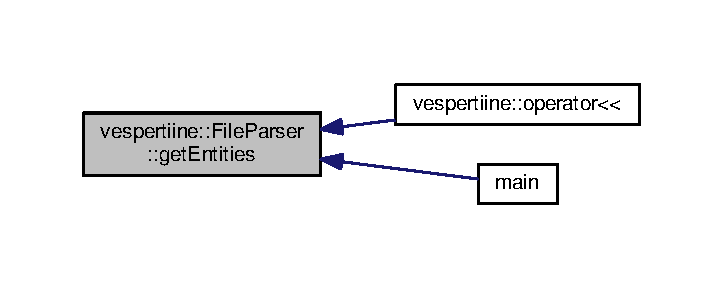
\includegraphics[width=347pt]{group__vespertiine_gac2360eb7febe37b75f13dc697a3d37ed_icgraph}
\end{center}
\end{figure}


\index{Vespertiine@{Vespertiine}!get\+File\+Type@{get\+File\+Type}}
\index{get\+File\+Type@{get\+File\+Type}!Vespertiine@{Vespertiine}}
\subsubsection[{\texorpdfstring{get\+File\+Type() const }{getFileType() const }}]{\setlength{\rightskip}{0pt plus 5cm}const string vespertiine\+::\+File\+Parser\+::get\+File\+Type (
\begin{DoxyParamCaption}
{}
\end{DoxyParamCaption}
) const}\hypertarget{group__vespertiine_ga950b19f6ead99d8297e37eaeeed2fd3f}{}\label{group__vespertiine_ga950b19f6ead99d8297e37eaeeed2fd3f}


Return the type of the file as a string. 

The string will be of the format, \char`\"{}\mbox{[}\+E\+N\+T\+I\+T\+Y\+\_\+\+T\+Y\+P\+E\mbox{]} \mbox{[}\+F\+I\+L\+E\+\_\+\+T\+Y\+P\+E\mbox{]}\char`\"{}.

\begin{DoxyReturn}{Returns}
The file type string. 
\end{DoxyReturn}


Definition at line 58 of file File\+Parser.\+cpp.



Here is the caller graph for this function\+:\nopagebreak
\begin{figure}[H]
\begin{center}
\leavevmode
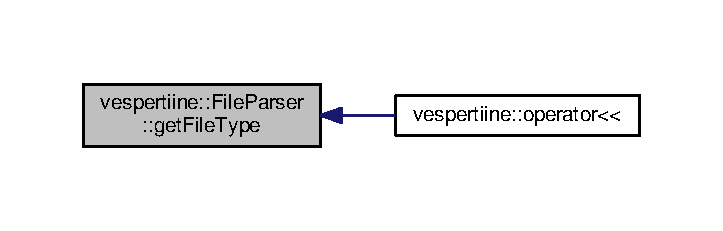
\includegraphics[width=347pt]{group__vespertiine_ga950b19f6ead99d8297e37eaeeed2fd3f_icgraph}
\end{center}
\end{figure}


\index{Vespertiine@{Vespertiine}!get\+File\+Version@{get\+File\+Version}}
\index{get\+File\+Version@{get\+File\+Version}!Vespertiine@{Vespertiine}}
\subsubsection[{\texorpdfstring{get\+File\+Version() const }{getFileVersion() const }}]{\setlength{\rightskip}{0pt plus 5cm}const unsigned int vespertiine\+::\+File\+Parser\+::get\+File\+Version (
\begin{DoxyParamCaption}
{}
\end{DoxyParamCaption}
) const}\hypertarget{group__vespertiine_ga69070e93ff23a24380d0bad1c096205a}{}\label{group__vespertiine_ga69070e93ff23a24380d0bad1c096205a}


Return the version of the file as a single unsigned integer. 

\begin{DoxyReturn}{Returns}
Version number of the file. 
\end{DoxyReturn}


Definition at line 57 of file File\+Parser.\+cpp.



Here is the caller graph for this function\+:\nopagebreak
\begin{figure}[H]
\begin{center}
\leavevmode
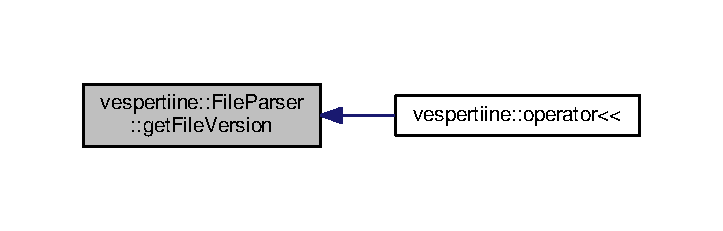
\includegraphics[width=347pt]{group__vespertiine_ga69070e93ff23a24380d0bad1c096205a_icgraph}
\end{center}
\end{figure}


\index{Vespertiine@{Vespertiine}!operator$<$$<$@{operator$<$$<$}}
\index{operator$<$$<$@{operator$<$$<$}!Vespertiine@{Vespertiine}}
\subsubsection[{\texorpdfstring{operator$<$$<$(std\+::ostream \&output, const vespertiine\+::\+File\+Parser \&\+F)}{operator<<(std::ostream &output, const vespertiine::FileParser &F)}}]{\setlength{\rightskip}{0pt plus 5cm}std\+::ostream\& vespertiine\+::operator$<$$<$ (
\begin{DoxyParamCaption}
\item[{std\+::ostream \&}]{output, }
\item[{const {\bf vespertiine\+::\+File\+Parser} \&}]{F}
\end{DoxyParamCaption}
)}\hypertarget{group__vespertiine_ga1ca507e4b8f52201ba9cccaaf496e9be}{}\label{group__vespertiine_ga1ca507e4b8f52201ba9cccaaf496e9be}
This will output a matching file similar to whatever is provided, however it will be alphabetically ordered by keys within each individual entity. 

Definition at line 60 of file File\+Parser.\+cpp.



Here is the call graph for this function\+:\nopagebreak
\begin{figure}[H]
\begin{center}
\leavevmode
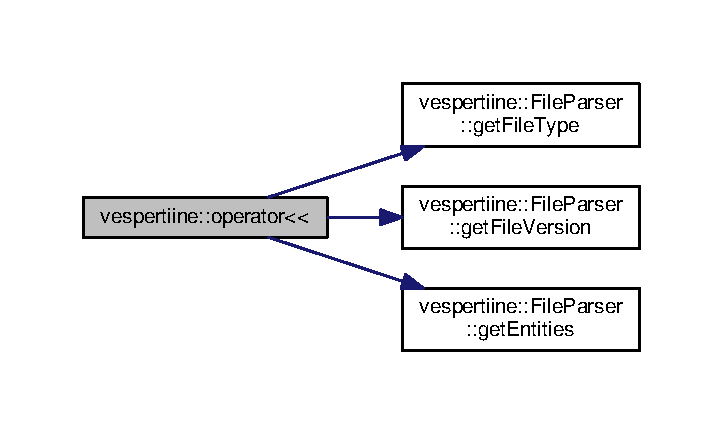
\includegraphics[width=347pt]{group__vespertiine_ga1ca507e4b8f52201ba9cccaaf496e9be_cgraph}
\end{center}
\end{figure}




\subsection{Friends}
\index{Vespertiine@{Vespertiine}!operator$<$$<$@{operator$<$$<$}}
\index{operator$<$$<$@{operator$<$$<$}!Vespertiine@{Vespertiine}}
\subsubsection[{\texorpdfstring{operator$<$$<$}{operator<<}}]{\setlength{\rightskip}{0pt plus 5cm}std\+::ostream\& operator$<$$<$ (
\begin{DoxyParamCaption}
\item[{std\+::ostream \&}]{output, }
\item[{const {\bf File\+Parser} \&}]{F}
\end{DoxyParamCaption}
)\hspace{0.3cm}{\ttfamily [friend]}}\hypertarget{group__vespertiine_ga6d174b85be314a05d54a9d63a7f1fbbb}{}\label{group__vespertiine_ga6d174b85be314a05d54a9d63a7f1fbbb}


Overload the output operator to match the style of the D\+IF type. 

This will output a matching file similar to whatever is provided, however it will be alphabetically ordered by keys within each individual entity. 

Definition at line 60 of file File\+Parser.\+cpp.


\chapter{Namespace Documentation}
\hypertarget{namespacevespertiine}{}\section{vespertiine Namespace Reference}
\label{namespacevespertiine}\index{vespertiine@{vespertiine}}
\subsection*{Classes}
\begin{DoxyCompactItemize}
\item 
class \hyperlink{classvespertiine_1_1FileParser}{File\+Parser}
\begin{DoxyCompactList}\small\item\em Parses C\+OM S 327 D\+IF files to a vector of maps of string pairs. \end{DoxyCompactList}\end{DoxyCompactItemize}
\subsection*{Typedefs}
\begin{DoxyCompactItemize}
\item 
using \hyperlink{group__vespertiine_ga7e5191e67b3b71f8044b653a3f9b2065}{string} = std\+::string
\item 
using \hyperlink{group__vespertiine_ga338498d8eeb1f5a3da1f237df24c4250}{istream} = std\+::istream
\item 
using \hyperlink{group__vespertiine_ga01f4e06d9363d6dc31a69d8a0553b93d}{entity\+\_\+vector} = std\+::vector$<$ \hyperlink{group__vespertiine_gaf9205d715bdeade18d7039864ef59b44}{entity} $>$
\item 
using \hyperlink{group__vespertiine_ga39a811996b190f9e1ffa0663d4f5744a}{file\+\_\+key} = std\+::string
\item 
using \hyperlink{group__vespertiine_ga546be9d1b39ff78c5bf63e598bc51a0a}{file\+\_\+value} = std\+::string
\item 
using \hyperlink{group__vespertiine_gaf9205d715bdeade18d7039864ef59b44}{entity} = std\+::map$<$ \hyperlink{group__vespertiine_ga39a811996b190f9e1ffa0663d4f5744a}{file\+\_\+key}, \hyperlink{group__vespertiine_ga546be9d1b39ff78c5bf63e598bc51a0a}{file\+\_\+value} $>$
\item 
using \hyperlink{group__vespertiine_ga1294ff353dd9ea9b26cf4a1573db109e}{file\+\_\+header} = std\+::pair$<$ std\+::string, unsigned int $>$
\end{DoxyCompactItemize}
\subsection*{Functions}
\begin{DoxyCompactItemize}
\item 
\hyperlink{group__vespertiine_ga338498d8eeb1f5a3da1f237df24c4250}{istream} \& \hyperlink{group__vespertiine_ga45bab8eea6e760c36a785c145af6ba25}{parseline} (\hyperlink{group__vespertiine_ga338498d8eeb1f5a3da1f237df24c4250}{istream} \&, \hyperlink{group__vespertiine_ga7e5191e67b3b71f8044b653a3f9b2065}{string} \&)
\item 
\hyperlink{group__vespertiine_ga338498d8eeb1f5a3da1f237df24c4250}{istream} \& \hyperlink{group__vespertiine_ga05687b76bc32ebfb4d97d92c417acaf6}{parseline} (\hyperlink{group__vespertiine_ga338498d8eeb1f5a3da1f237df24c4250}{istream} \&, \hyperlink{group__vespertiine_ga7e5191e67b3b71f8044b653a3f9b2065}{string} \&, char $\ast$)
\item 
\hyperlink{group__vespertiine_ga7e5191e67b3b71f8044b653a3f9b2065}{string} \hyperlink{group__vespertiine_ga5541b037e75ed830f526c2e073b26474}{trim} (\hyperlink{group__vespertiine_ga7e5191e67b3b71f8044b653a3f9b2065}{string})
\item 
std\+::ostream \& \hyperlink{group__vespertiine_ga1ca507e4b8f52201ba9cccaaf496e9be}{operator$<$$<$} (std\+::ostream \&output, const \hyperlink{classvespertiine_1_1FileParser}{vespertiine\+::\+File\+Parser} \&F)
\end{DoxyCompactItemize}

\chapter{Class Documentation}
\hypertarget{classvespertiine_1_1FileParser}{}\section{vespertiine\+:\+:File\+Parser Class Reference}
\label{classvespertiine_1_1FileParser}\index{vespertiine\+::\+File\+Parser@{vespertiine\+::\+File\+Parser}}


Parses C\+OM S 327 D\+IF files to a vector of maps of string pairs.  




{\ttfamily \#include $<$File\+Parser.\+hpp$>$}

\subsection*{Public Member Functions}
\begin{DoxyCompactItemize}
\item 
\hyperlink{group__vespertiine_ga01e372573c11d4c2848419c8842d583e}{File\+Parser} (std\+::string file\+\_\+path)
\begin{DoxyCompactList}\small\item\em Construct and populate the \hyperlink{classvespertiine_1_1FileParser}{File\+Parser}. \end{DoxyCompactList}\item 
const std\+::vector$<$ \hyperlink{group__vespertiine_gaf9205d715bdeade18d7039864ef59b44}{entity} $>$ \hyperlink{group__vespertiine_gac2360eb7febe37b75f13dc697a3d37ed}{get\+Entities} () const 
\begin{DoxyCompactList}\small\item\em Return the contents of the file. \end{DoxyCompactList}\item 
const unsigned int \hyperlink{group__vespertiine_ga69070e93ff23a24380d0bad1c096205a}{get\+File\+Version} () const 
\begin{DoxyCompactList}\small\item\em Return the version of the file as a single unsigned integer. \end{DoxyCompactList}\item 
const std\+::string \hyperlink{group__vespertiine_ga950b19f6ead99d8297e37eaeeed2fd3f}{get\+File\+Type} () const 
\begin{DoxyCompactList}\small\item\em Return the type of the file as a string. \end{DoxyCompactList}\end{DoxyCompactItemize}
\subsection*{Friends}
\begin{DoxyCompactItemize}
\item 
std\+::ostream \& \hyperlink{group__vespertiine_ga6d174b85be314a05d54a9d63a7f1fbbb}{operator$<$$<$} (std\+::ostream \&output, const \hyperlink{classvespertiine_1_1FileParser}{File\+Parser} \&F)
\begin{DoxyCompactList}\small\item\em Overload the output operator to match the style of the D\+IF type. \end{DoxyCompactList}\end{DoxyCompactItemize}


\subsection{Detailed Description}
Parses C\+OM S 327 D\+IF files to a vector of maps of string pairs. 

The constructor expects a string of a filepath. The file can be parsed under the following assumptions\+:
\begin{DoxyEnumerate}
\item Possess a header on the first line of the format \char`\"{}\+R\+L\+G327 \mbox{[}entity\+\_\+type\mbox{]} \mbox{[}file\+\_\+type\mbox{]} \mbox{[}version\+\_\+number\mbox{]}\char`\"{}
\item Possess entities wrapped in B\+E\+G\+IN \mbox{[}E\+N\+T\+I\+T\+Y\+\_\+\+N\+A\+ME\mbox{]} ... E\+ND tags on their own lines.
\item Possess keys of at least two capital letters followed by a newline or a value. 3a. If followed by a newline, the multiline values must end with a \mbox{[}.\mbox{]} on its own line.
\end{DoxyEnumerate}

\begin{DoxyAuthor}{Author}
Freya Gaynor 
\end{DoxyAuthor}
\begin{DoxyDate}{Date}
2018-\/03-\/28 
\end{DoxyDate}


Definition at line 32 of file File\+Parser.\+hpp.



The documentation for this class was generated from the following files\+:\begin{DoxyCompactItemize}
\item 
src/include/\hyperlink{FileParser_8hpp}{File\+Parser.\+hpp}\item 
src/\hyperlink{FileParser_8cpp}{File\+Parser.\+cpp}\end{DoxyCompactItemize}

\chapter{File Documentation}
\hypertarget{FileParser_8cpp}{}\section{src/\+File\+Parser.cpp File Reference}
\label{FileParser_8cpp}\index{src/\+File\+Parser.\+cpp@{src/\+File\+Parser.\+cpp}}
{\ttfamily \#include $<$functional$>$}\\*
{\ttfamily \#include \char`\"{}File\+Parser.\+hpp\char`\"{}}\\*
Include dependency graph for File\+Parser.\+cpp\+:
\nopagebreak
\begin{figure}[H]
\begin{center}
\leavevmode
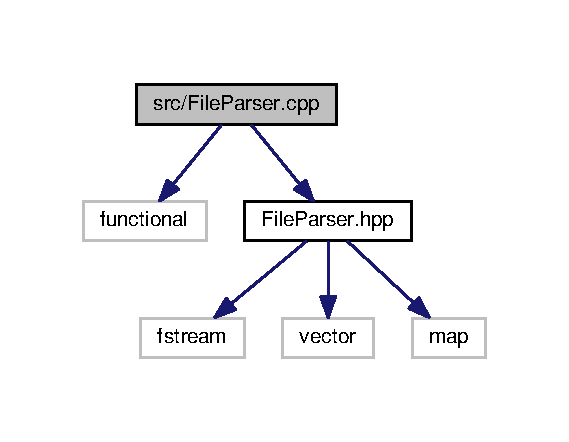
\includegraphics[width=273pt]{FileParser_8cpp__incl}
\end{center}
\end{figure}
\subsection*{Namespaces}
\begin{DoxyCompactItemize}
\item 
 \hyperlink{namespacevespertiine}{vespertiine}
\end{DoxyCompactItemize}
\subsection*{Typedefs}
\begin{DoxyCompactItemize}
\item 
using \hyperlink{group__vespertiine_ga7e5191e67b3b71f8044b653a3f9b2065}{vespertiine\+::string} = std\+::string
\item 
using \hyperlink{group__vespertiine_ga338498d8eeb1f5a3da1f237df24c4250}{vespertiine\+::istream} = std\+::istream
\item 
using \hyperlink{group__vespertiine_ga01f4e06d9363d6dc31a69d8a0553b93d}{vespertiine\+::entity\+\_\+vector} = std\+::vector$<$ entity $>$
\end{DoxyCompactItemize}
\subsection*{Functions}
\begin{DoxyCompactItemize}
\item 
istream \& \hyperlink{group__vespertiine_ga45bab8eea6e760c36a785c145af6ba25}{vespertiine\+::parseline} (istream \&, string \&)
\item 
istream \& \hyperlink{group__vespertiine_ga05687b76bc32ebfb4d97d92c417acaf6}{vespertiine\+::parseline} (istream \&, string \&, char $\ast$)
\item 
string \hyperlink{group__vespertiine_ga5541b037e75ed830f526c2e073b26474}{vespertiine\+::trim} (string)
\item 
std\+::ostream \& \hyperlink{group__vespertiine_ga1ca507e4b8f52201ba9cccaaf496e9be}{vespertiine\+::operator$<$$<$} (std\+::ostream \&output, const \hyperlink{classvespertiine_1_1FileParser}{vespertiine\+::\+File\+Parser} \&F)
\end{DoxyCompactItemize}


\subsection{Detailed Description}
\begin{DoxyAuthor}{Author}
Freya Gaynor 
\end{DoxyAuthor}
\begin{DoxyDate}{Date}
2018-\/03-\/28
\end{DoxyDate}
A modular file parser for C\+OM S 327 wtih Dr. Shaeffer. 
\hypertarget{FileParser_8hpp}{}\section{src/include/\+File\+Parser.hpp File Reference}
\label{FileParser_8hpp}\index{src/include/\+File\+Parser.\+hpp@{src/include/\+File\+Parser.\+hpp}}
{\ttfamily \#include $<$fstream$>$}\\*
{\ttfamily \#include $<$vector$>$}\\*
{\ttfamily \#include $<$map$>$}\\*
Include dependency graph for File\+Parser.\+hpp\+:\nopagebreak
\begin{figure}[H]
\begin{center}
\leavevmode
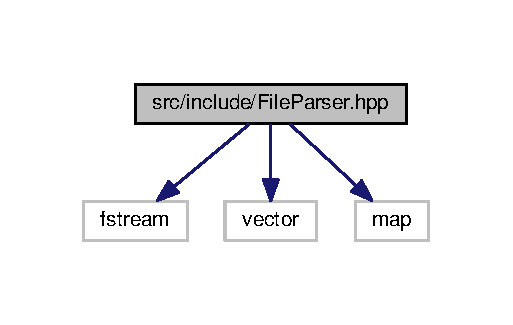
\includegraphics[width=246pt]{FileParser_8hpp__incl}
\end{center}
\end{figure}
This graph shows which files directly or indirectly include this file\+:\nopagebreak
\begin{figure}[H]
\begin{center}
\leavevmode
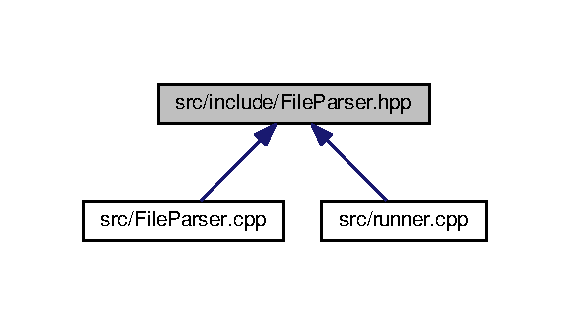
\includegraphics[width=274pt]{FileParser_8hpp__dep__incl}
\end{center}
\end{figure}
\subsection*{Classes}
\begin{DoxyCompactItemize}
\item 
class \hyperlink{classvespertiine_1_1FileParser}{vespertiine\+::\+File\+Parser}
\begin{DoxyCompactList}\small\item\em Parses C\+OM S 327 D\+IF files to a vector of maps of string pairs. \end{DoxyCompactList}\end{DoxyCompactItemize}
\subsection*{Namespaces}
\begin{DoxyCompactItemize}
\item 
 \hyperlink{namespacevespertiine}{vespertiine}
\end{DoxyCompactItemize}
\subsection*{Typedefs}
\begin{DoxyCompactItemize}
\item 
using \hyperlink{group__vespertiine_ga39a811996b190f9e1ffa0663d4f5744a}{vespertiine\+::file\+\_\+key} = std\+::string
\item 
using \hyperlink{group__vespertiine_ga546be9d1b39ff78c5bf63e598bc51a0a}{vespertiine\+::file\+\_\+value} = std\+::string
\item 
using \hyperlink{group__vespertiine_gaf9205d715bdeade18d7039864ef59b44}{vespertiine\+::entity} = std\+::map$<$ file\+\_\+key, file\+\_\+value $>$
\item 
using \hyperlink{group__vespertiine_ga1294ff353dd9ea9b26cf4a1573db109e}{vespertiine\+::file\+\_\+header} = std\+::pair$<$ std\+::string, unsigned int $>$
\end{DoxyCompactItemize}

\hypertarget{runner_8cpp}{}\section{src/runner.cpp File Reference}
\label{runner_8cpp}\index{src/runner.\+cpp@{src/runner.\+cpp}}
{\ttfamily \#include $<$iostream$>$}\\*
{\ttfamily \#include $<$algorithm$>$}\\*
{\ttfamily \#include \char`\"{}File\+Parser.\+hpp\char`\"{}}\\*
Include dependency graph for runner.\+cpp\+:
\nopagebreak
\begin{figure}[H]
\begin{center}
\leavevmode
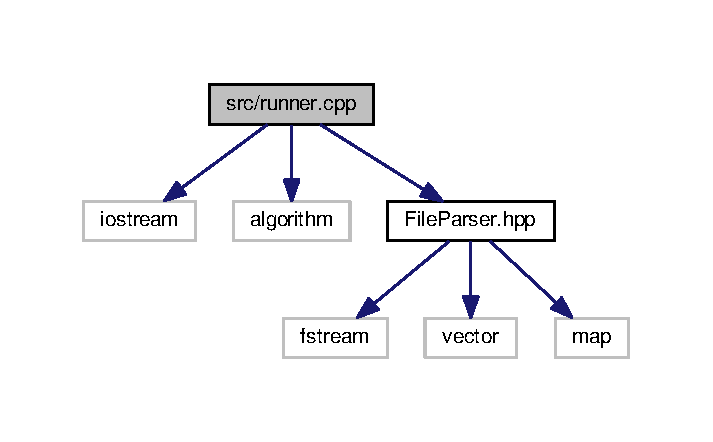
\includegraphics[width=342pt]{runner_8cpp__incl}
\end{center}
\end{figure}
\subsection*{Functions}
\begin{DoxyCompactItemize}
\item 
int \hyperlink{runner_8cpp_abf9e6b7e6f15df4b525a2e7705ba3089}{main} (int argc, char const $\ast$argv\mbox{[}$\,$\mbox{]})
\end{DoxyCompactItemize}


\subsection{Function Documentation}
\index{runner.\+cpp@{runner.\+cpp}!main@{main}}
\index{main@{main}!runner.\+cpp@{runner.\+cpp}}
\subsubsection[{\texorpdfstring{main(int argc, char const $\ast$argv[])}{main(int argc, char const *argv[])}}]{\setlength{\rightskip}{0pt plus 5cm}int main (
\begin{DoxyParamCaption}
\item[{int}]{argc, }
\item[{char const $\ast$}]{argv\mbox{[}$\,$\mbox{]}}
\end{DoxyParamCaption}
)}\hypertarget{runner_8cpp_abf9e6b7e6f15df4b525a2e7705ba3089}{}\label{runner_8cpp_abf9e6b7e6f15df4b525a2e7705ba3089}


Definition at line 4 of file runner.\+cpp.



Here is the call graph for this function\+:
\nopagebreak
\begin{figure}[H]
\begin{center}
\leavevmode
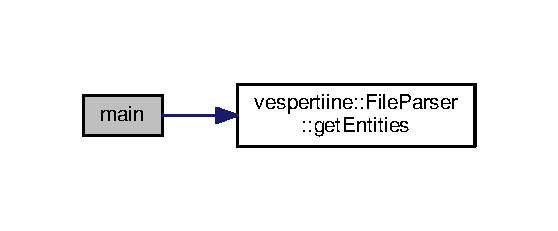
\includegraphics[width=268pt]{runner_8cpp_abf9e6b7e6f15df4b525a2e7705ba3089_cgraph}
\end{center}
\end{figure}



%--- End generated contents ---

% Index
\backmatter
\newpage
\phantomsection
\clearemptydoublepage
\addcontentsline{toc}{chapter}{Index}
\printindex

\end{document}
